\documentclass[aspectratio=169,14pt]{beamer}
\usepackage[utf8]{inputenc}
\usepackage{minted}
\usepackage{listings}
\usepackage[normalem]{ulem}
\usetheme{veit}
\title{Memory Vulnerabilities in Memory-safe Languages}
\date{\today}
\author{Veit Heller}
\institute{Information Security Meetup Berlin, August 2020}
\begin{document}
  \maketitle
  \section{Scope}
  \begin{frame}{Scope}
    \sout{Compilers/Interpreters}
  \end{frame}
  \begin{frame}{Python}
    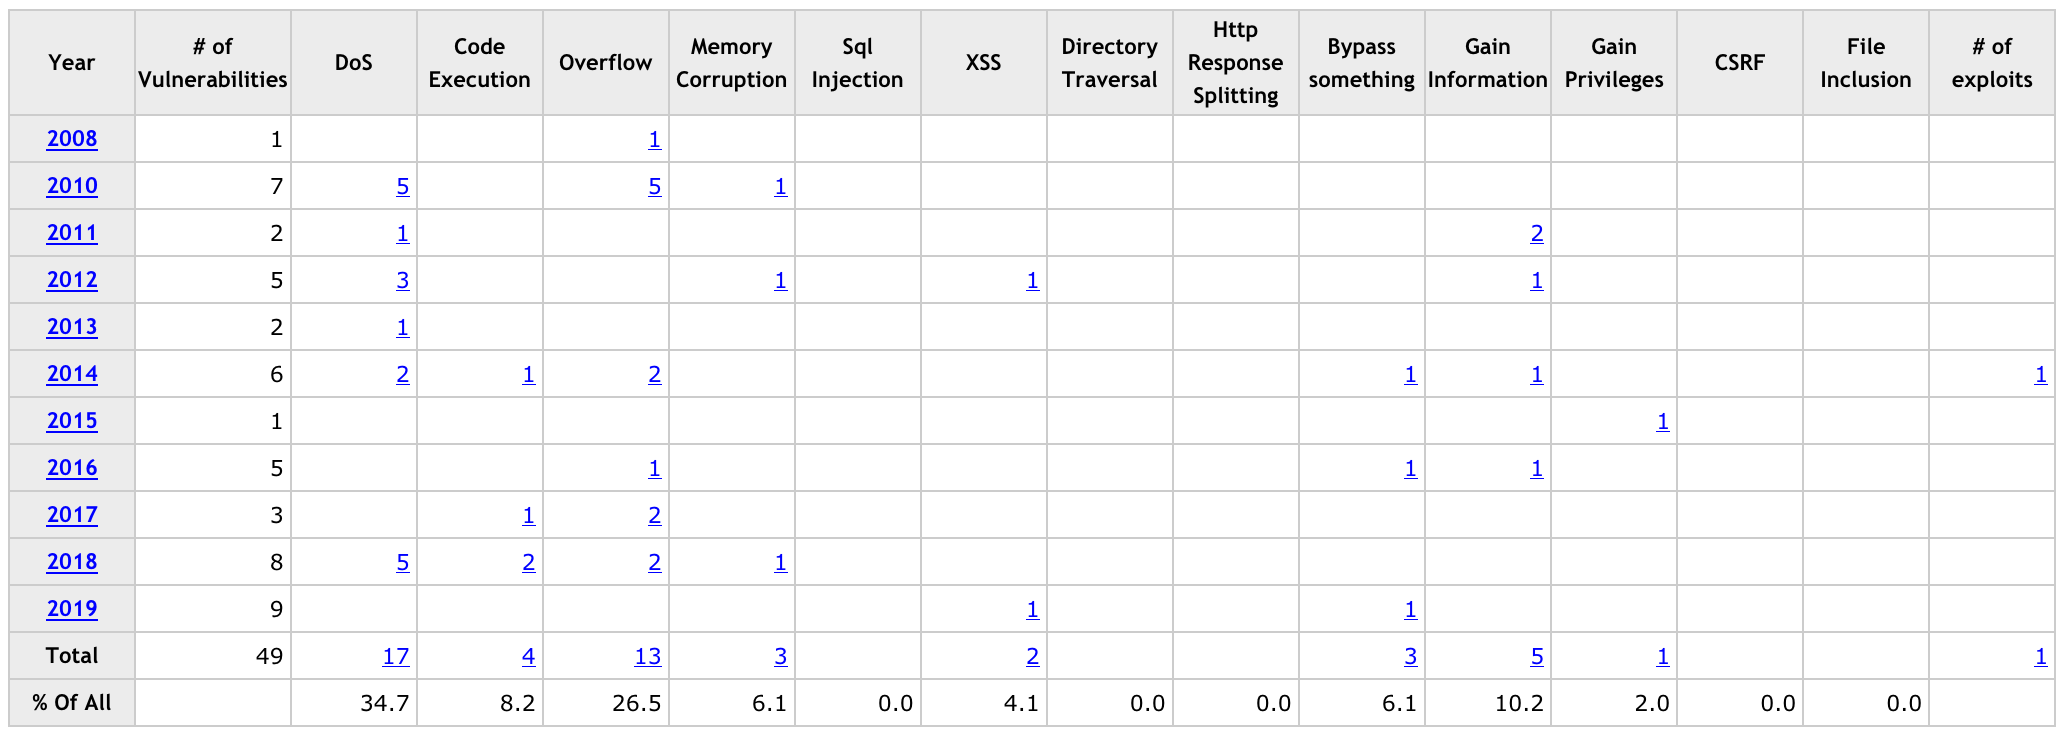
\includegraphics[width=14cm]{python_cves}
  \end{frame}
  \begin{frame}{JavaScript}
    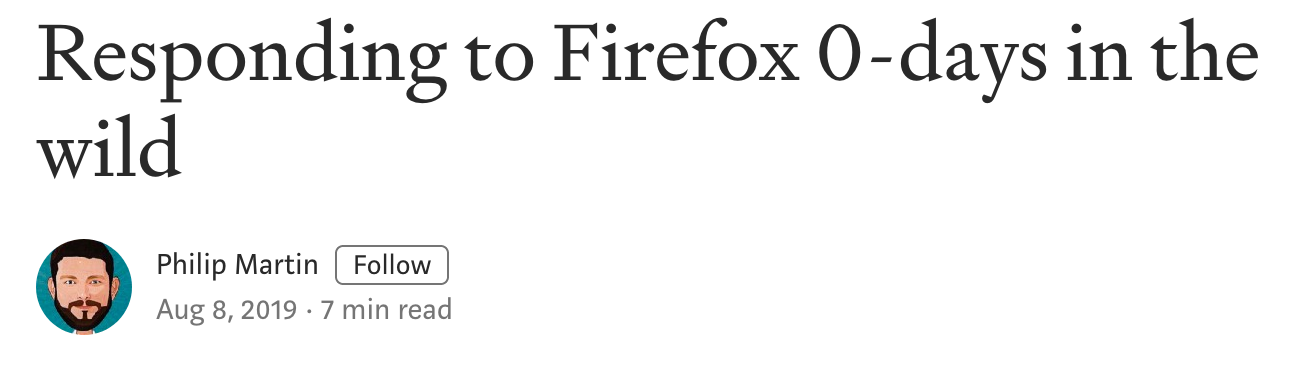
\includegraphics[width=14cm]{js_1}
  \end{frame}
  \begin{frame}{JavaScript...}
    
\includegraphics[width=14cm]{js_2}
  \end{frame}
  \begin{frame}{More JavaScript...}
    
\includegraphics[width=14cm]{js_3}
  \end{frame}
  \begin{frame}{Scope}
    Runtimes
  \end{frame}
  \begin{frame}{Scope}
    \sout{Bashing}
  \end{frame}
  \begin{frame}{Scope}
    \sout{Bashing}

    $\Rightarrow$ No Silver Bullets
  \end{frame}
  \section{Denial of Service (DoS)}
  \begin{frame}{Concurrency}
    Concurrency is getting easier to work with.
  \end{frame}
  \begin{frame}{Concurrency}
    When something is easy to work with, we tend to shoot ourselves in the
    foot with it.
  \end{frame}
  \begin{frame}{Concurrency}
    Let’s talk about channels.
  \end{frame}
  \begin{frame}{Concurrency}
    If a value is written to a channel and never read, what happens to it?
  \end{frame}
  \begin{frame}{Concurrency}
    What happens if we wait to read and noone answers?
  \end{frame}
  \begin{frame}{Concurrency}
    Always think about your processes’ lifetimes.
  \end{frame}
  \begin{frame}{Go issue 20135}
    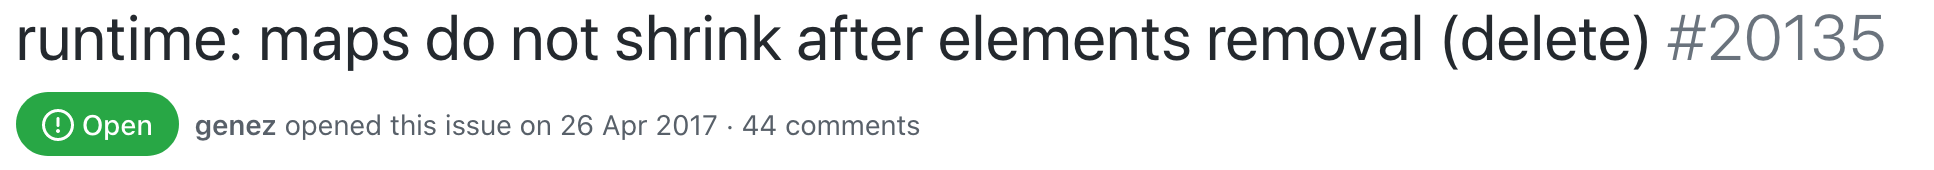
\includegraphics[width=14cm]{go_20135}
  \end{frame}
  \begin{frame}[fragile]
    \frametitle{Go issue 20135}
    \begin{listing}[H]
      \caption{Go sitting on your memory.}
      \begin{minted}[fontsize=\footnotesize]{go}
func main() {
  runtime.GC(); memUsage() // basically 0
  m := make(map[int]int)  // we start alloc’ing

  for i := 0; i < 100000; i++ { m[i] = i }

  runtime.GC() // nothing deleted, of course

  for i := 0; i < 100000; i++ { delete(m, i) }

  runtime.GC() // still nothing deleted!

  fmt.Println(m) // just to make sure GC is not too clever
}
      \end{minted}
    \end{listing}
  \end{frame}
  \begin{frame}{So?}
    \begin{itemize}
      \item Memory bugs don’t need to corrupt memory.
    \end{itemize}
  \end{frame}
  \begin{frame}{So?}
    \begin{itemize}
      \item Memory bugs don’t need to corrupt memory.
      \item Runtimes hide a lot from you (good and bad).
    \end{itemize}
  \end{frame}
  \begin{frame}{Haskell}
    Haskell is lazy.
  \end{frame}
  \begin{frame}[fragile]
    \frametitle{Haskell}
    \begin{listing}[H]
      \caption{Thunks in action.}
      \begin{minted}{haskell}
let (x, y) = (1 + 2, error "boom!") in x -- => 3
      \end{minted}
    \end{listing}
  \end{frame}
  \begin{frame}{Haskell}
    \begin{center}
      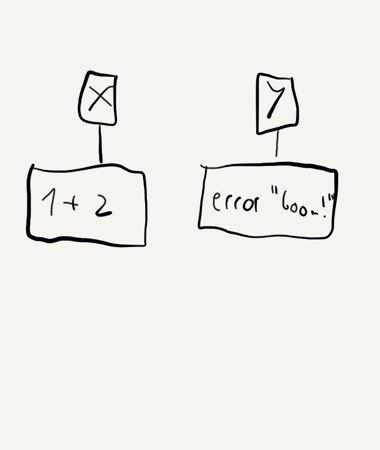
\includegraphics[width=6cm]{lazy_before}
    \end{center}
  \end{frame}
  \begin{frame}{Haskell}
    \begin{center}
      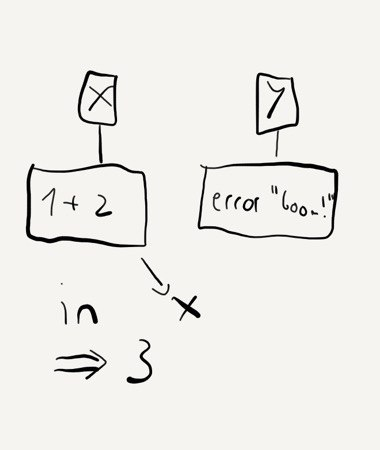
\includegraphics[width=6cm]{lazy_after}
    \end{center}
  \end{frame}
  \begin{frame}{Haskell}
    New vocabulary: space leaks.
  \end{frame}
  \begin{frame}{Space Leaks}
    ``Pinpointing spayce leaks is a skill that takes practice and perseverance. Better
    tools could significantly simplify the process.``

    --- Mitchell, Neil: Leaking Space. Eliminating memory hogs.
  \end{frame}
  \begin{frame}{Space Leaks}
    ``Using the benchmark I observed a space leak. But the program is huge, and
    manual code inspection usually needs a 10 line code fragment to have a change.
    So I started modifying the program to do less, and continued until the program
    did as little as it could, but still leaked space. After I fixed a space leak,
    I zoomed out and saw if the space leak persisted, and then had another go.``

    --- Mitchell, Neil: Fixing Space Leaks in Ghcide
  \end{frame}
  \begin{frame}{So?}
    \begin{itemize}
      \item Again: Runtimes hide a lot from you (good and bad).
    \end{itemize}
  \end{frame}
  \begin{frame}{So?}
    \begin{itemize}
      \item Again: Runtimes hide a lot from you (good and bad).
      \item If your runtime is complex, it can feel like an adversary.
    \end{itemize}
  \end{frame}
  \section{Memory Bugs}
  \begin{frame}[fragile]
    \frametitle{Rust}
    \begin{listing}[H]
      \caption{\texttt{unsafe} considered... unsafe?}
      \begin{minted}[fontsize=\small]{rust}
fn main() {
  unsafe fn dangerous<'a>() -> *const String {
    let tmp:String = "boom goes the dynamite!".to_string();
    &tmp
  }

  println!("{:?}", unsafe { dangerous().as_ref() })
}
      \end{minted}
    \end{listing}
  \end{frame}
  \begin{frame}{Rust}
    \texttt{\#![\,forbid(unsafe\_code)]\,}
  \end{frame}
  \begin{frame}{Rust}
    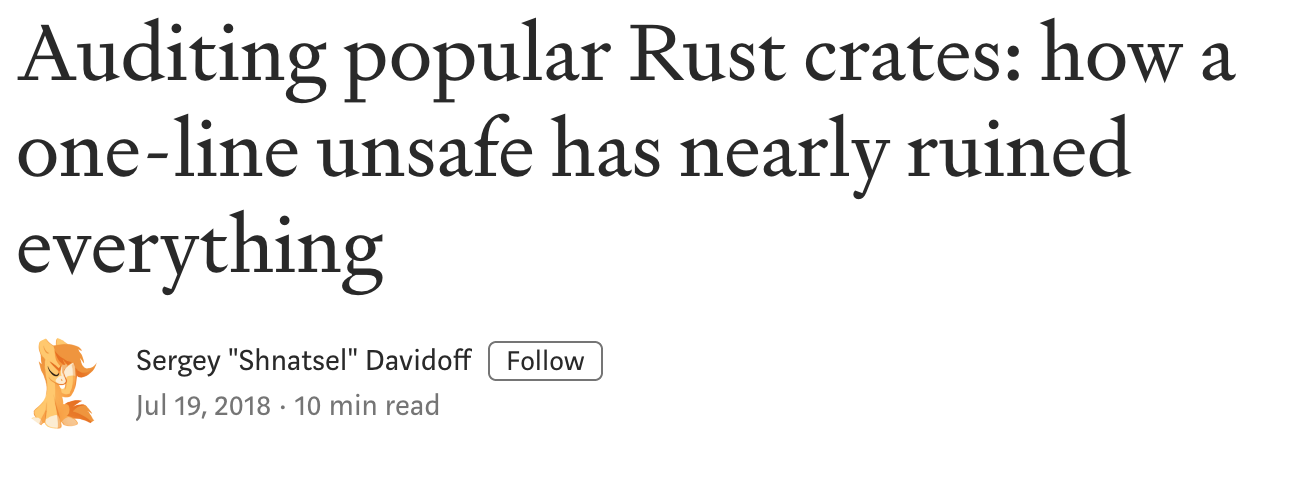
\includegraphics[width=14cm]{auditing_rust_crates}
  \end{frame}
  \begin{frame}{Rust}
    ``If you want to write DoS-critical code in Rust and use some existing
    libraries, you’re out of luck. Nobody cares about denial of service attacks.
    You can poke popular crates with a uzzer and get lots of those. When you report them, they do not get fixed.``

    --- Davidoff, Sergey (Shnatsel): How Rust’s standard library was vulnerable for years and nobody noticed
  \end{frame}
  \begin{frame}{Rust}
    
\includegraphics[width=12cm]{rust_memory}
  \end{frame}
  \begin{frame}{Rust}
  ``Most importantly, we find while Rust successfully limits memory-safety risks to
  the realm of unsafe code, it also brings some side effects that cause new
  patterns of dangling-pointer issues. In particular, most of the use-after-free
  and double-free bugs are related to the automatic destruction mechanism
  associated with the ownership-based memory management scheme.``

  --- Xu, Hui et al.: Memory-Safety Challenge Considered Solved? An In-Depth Experience Report with All Rust CVEs
  \end{frame}
  \begin{frame}{So?}
    \begin{itemize}
      \item Don’t use your language’s escape hatches.
    \end{itemize}
  \end{frame}
  \begin{frame}{So?}
    \begin{itemize}
      \item Don’t use your language’s escape hatches.
      \item Seriously.
    \end{itemize}
  \end{frame}
  \begin{frame}{So?}
    \begin{itemize}
      \item Don’t use your language’s escape hatches.
      \item Seriously.
      \item Please.
    \end{itemize}
  \end{frame}
  \begin{frame}{So?}
    \begin{itemize}
      \item Don’t use your language’s escape hatches.
      \item Seriously.
      \item Please.
      \item Or write proofs, but I know you won’t, so don’t.
    \end{itemize}
  \end{frame}
  \section{Conclusions (and better vibes)}
  \begin{frame}{Conclusion}
    Everything sucks in its own way, and that’s alright.
  \end{frame}
  \begin{frame}{Conclusion}
    Nothing will be perfectly secure. Make a better threat model.
  \end{frame}
  \begin{frame}{References}
    \begin{itemize}
      \item These slides: \texttt{https://github.com/hellerve/talks}
      \item Go bug 20135: \texttt{https://github.com/golang/go/issues/20135}
      \item Breaking Erlang Maps: \texttt{https://medium.com/@jlouis666/breaking-erlang-maps-1-31952b8729e6}
      \item RustBelt: \texttt{https://plv.mpi-sws.org/rustbelt}
      \item Space leak: A Haskell Sore Spot: \texttt{https://fremissant.net/leaky}
      \item Auditing popular Rust crates: how a one-line unsafe has nearly ruined everything: \texttt{https://medium.com/@shnatsel/auditing-popular-rust-crates-how-a-one-line-unsafe-has-nearly-ruined-everything-fab2d837ebb1}
      \item Fixing Space Leaks in Ghcide: \texttt{https://neilmitchell.blogspot.com/2020/05/fixing-space-leaks-in-ghcide.html}
    \end{itemize}
  \end{frame}
  \begin{frame}{References}
    \begin{itemize}
      \item Apple Paid Hacker 75,000 for Uncovering Zero-Day Camera Exploits in Safari \texttt{https://www.macrumors.com/2020/04/03/apple-paid-hacker-camera-exploits-safari/}
      \item Google patches Chrome zero-day under active attacks \texttt{https://www.zdnet.com/article/google-patches-chrome-zero-day-under-active-attacks/}
      \item Responding to Firefox 0-days in the wild \texttt{https://blog.coinbase.com/responding-to-firefox-0-days-in-the-wild-d9c85a57f15b}
      \item Xu, Hui et al.: Memory-Safety Challenge Considered Solved? An In-Depth Experience Report with All Rust CVEs
      \item Kulal, Sumith et al.: Space leaks exploration in Haskell
      \item Mitchell, Neil: Leaking Space—Eliminating memory hogs
    \end{itemize}
  \end{frame}
  \begin{frame}{}
    Thank you!

    \bigskip

    Questions?

    \bigskip

    \tiny Slides at \texttt{https://github.com/hellerve/talks}
  \end{frame}
\end{document}
